\subsubsection{Stratégie de décodage}

La sortie de la dernière couche du transformeur est une loi de probabilité sur le vocabulaire de \(L_C\) 
(voir Figure~\ref{fig.transformer2}).
À fin d'obtenir une phrase, le décodeur est appelé autorégressivement avec la phrase vide comme grain.
À chaque étape, il génère un mot en utilisant la loi de probabilité.
Ce mot est ajouté à la phrase et le décodeur est appelé récursivement avec la phrase ainsi obtenue.
Ce processus est répété jusqu'à ce que le symbole de fin de phrase soit généré~\cite{attention}.

Plusieurs méthodes existent pour générer un mot à partir de la loi de probabilité.
La plus simple est de choisir le mot qui a la plus grande probabilité,
on parle alors de décodage glouton, décodage \(\argmax\) ou décodage par maximum a posteriori.

\begin{figure}[hbt]
    \centering
    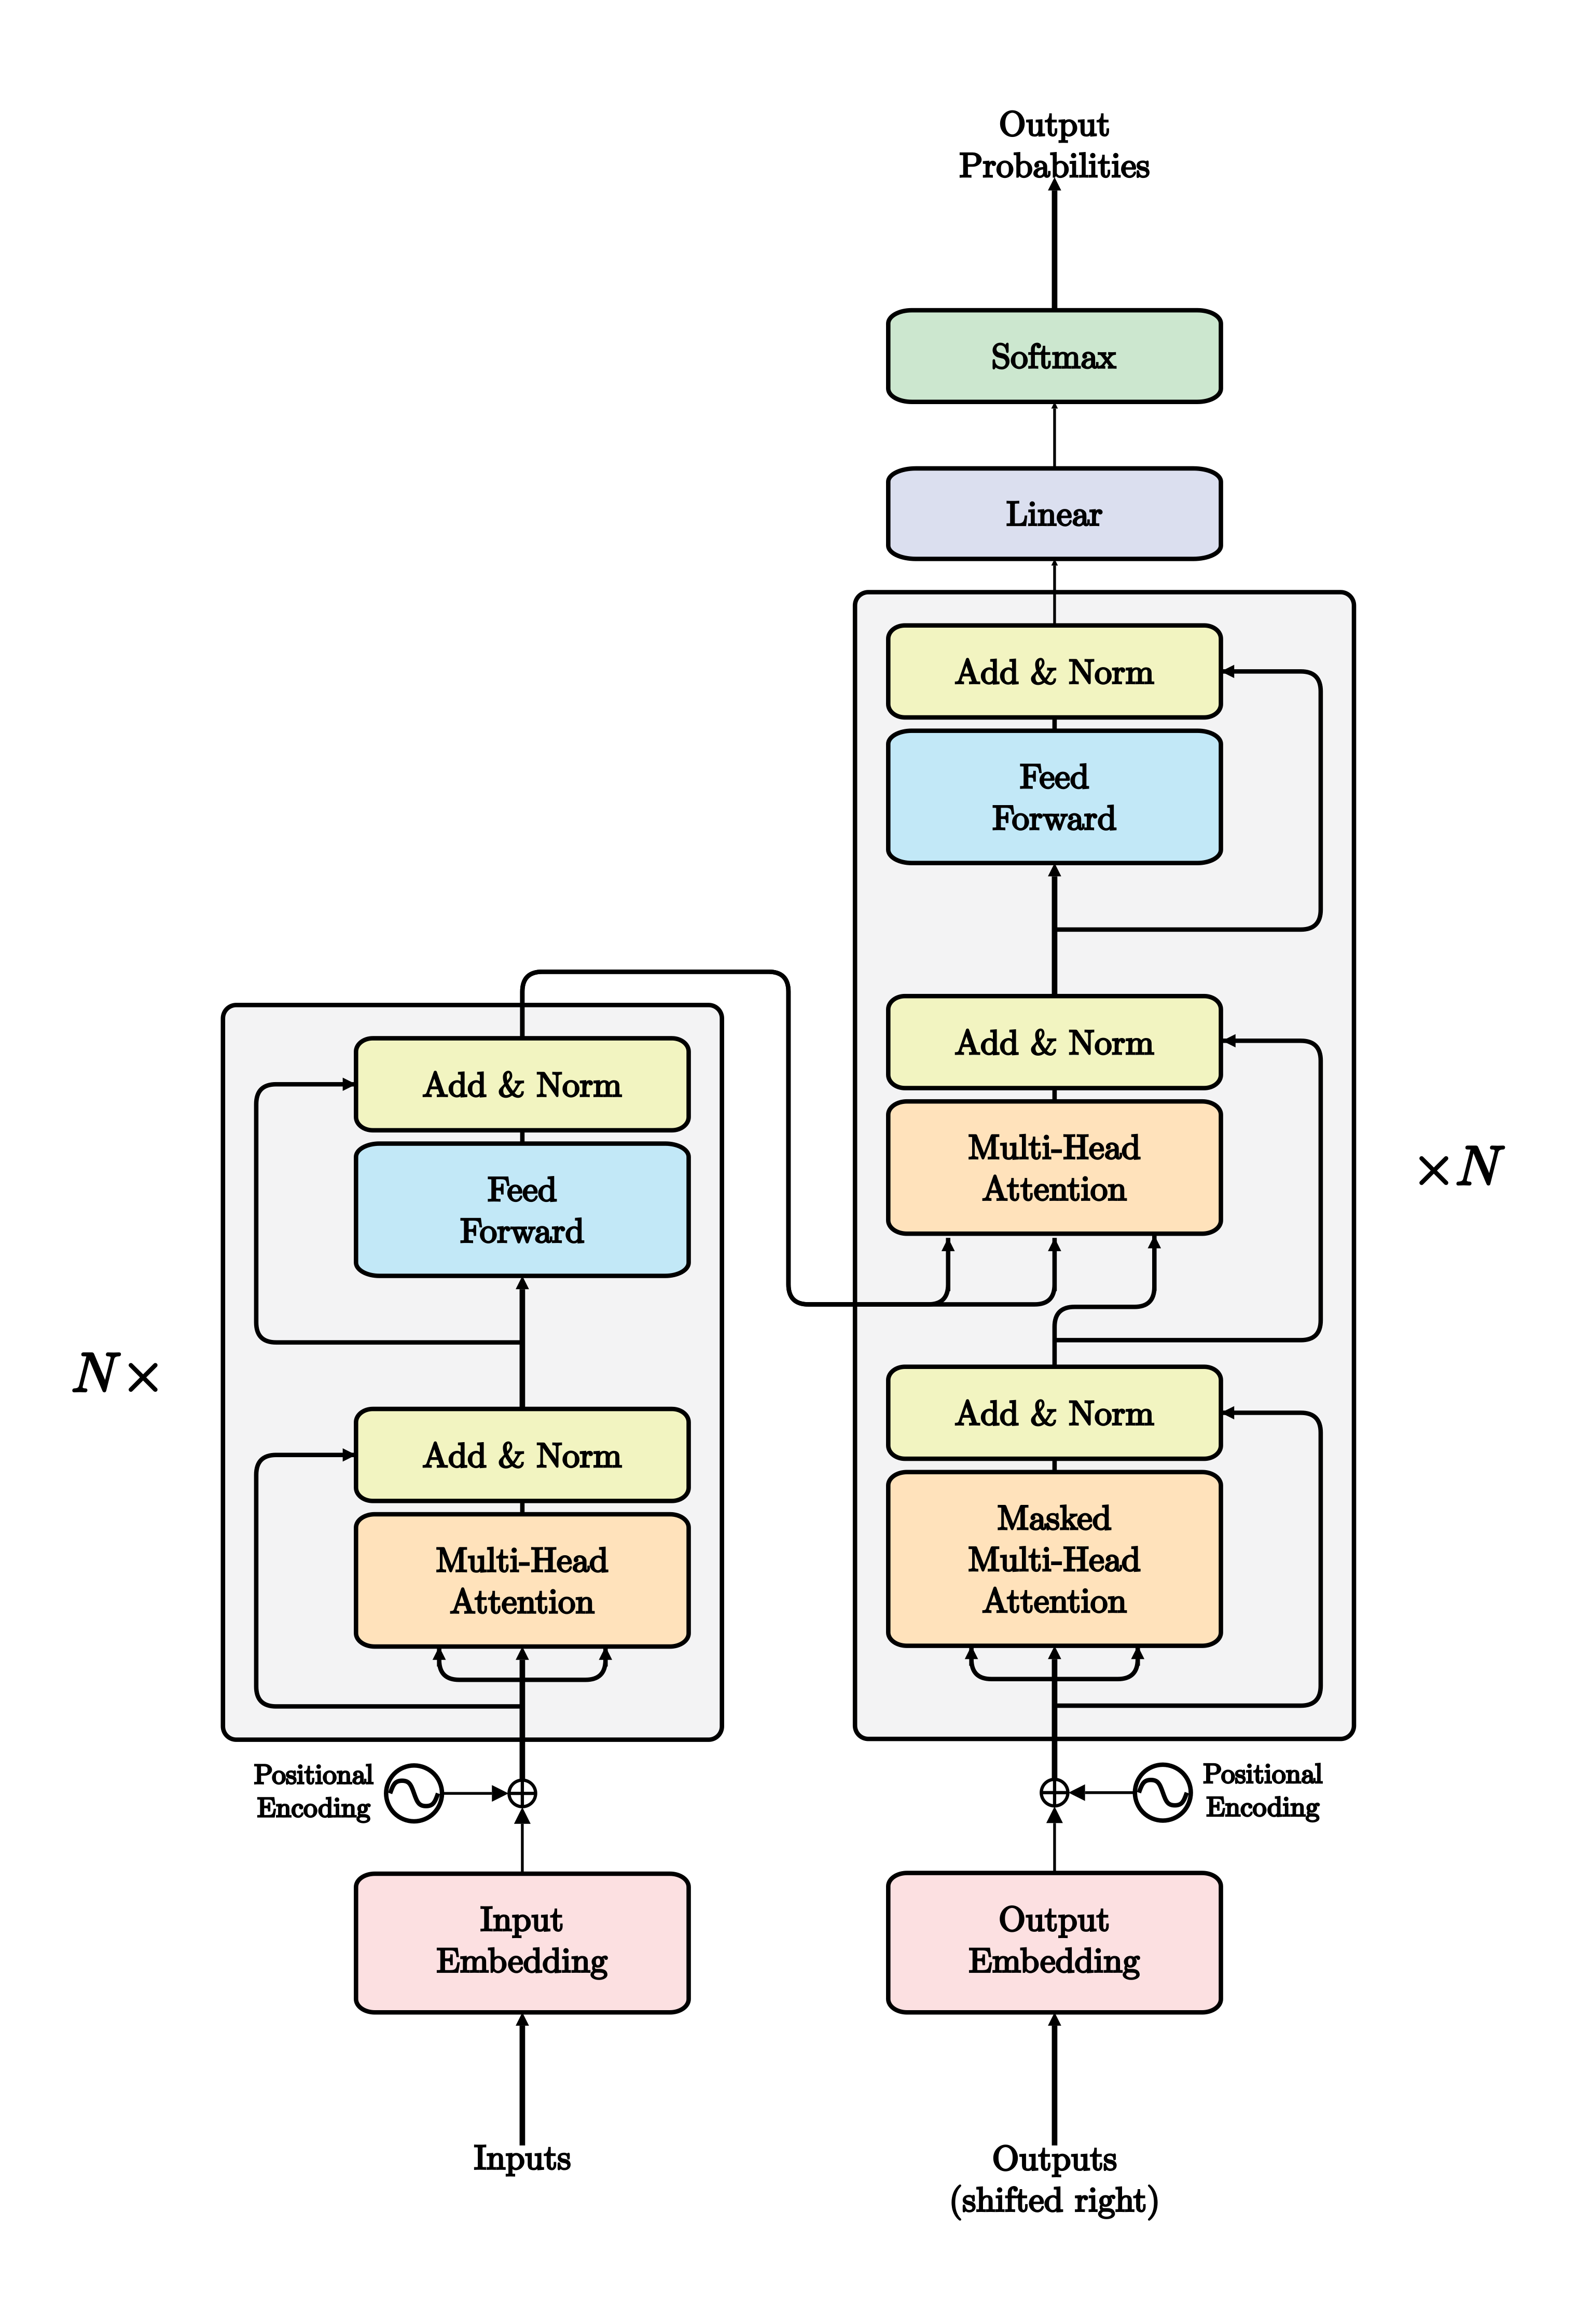
\includegraphics[width=8cm]{assets/images/transformer.png}
    \caption[L'architecture de transformeur.]
    {Architecture de transformeur~\cite{attention}.}
    \label{fig.transformer2}
\end{figure}

Cependant, cette méthode est suboptimale.
L'alternative la plus courante est ce qu'on appelle le décodage \emph{\foreignlanguage{english}{beam search}}%
~\cite{Meister_Vieira_Cotterell_2021}.

\lstinputlisting[
    language=Python, 
    caption={Passe d'un \glsfmtshort{mlp}}, 
    label={algo.bs-decode},
]{assets/code/bs-decode.py}